\section{Question I}
\subsection{Perceptron Algorithm}

Performance on training set: 0.5598 \\
Performance on validation set: 0.3868 \\
Performance on test set: 0.3743 \\

\begin{figure}[H]
    \centering
    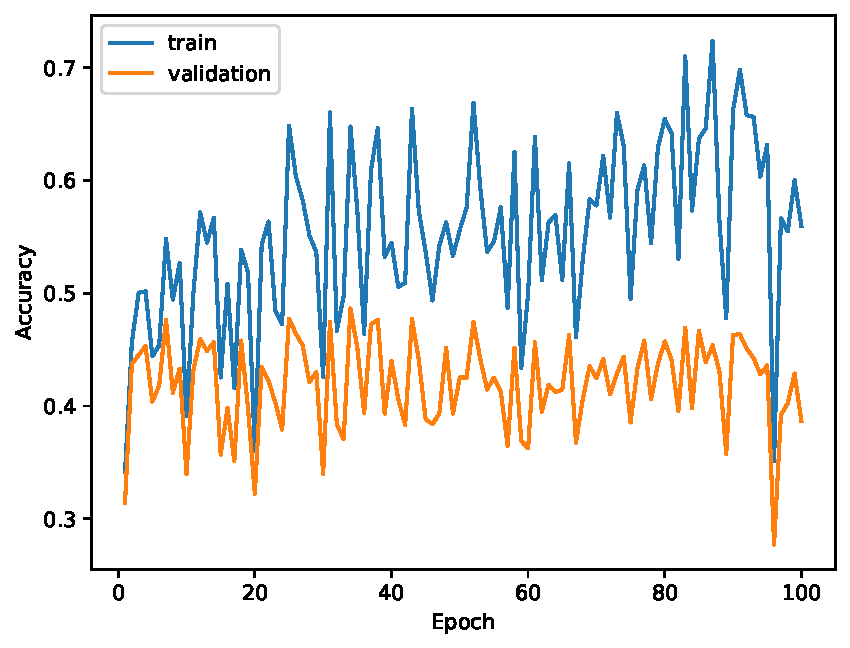
\includegraphics[width=0.4\textwidth]{images/Q1-perceptron-accs.pdf} 
    \caption{Train and validation accuracies for the Perceptron}
    \label{fig:dd}
\end{figure}



\subsection{Logistic Regression}
Accuracies obtained without regularization: \\
Performance on training set: 0.6694 \\
Performance on validation set: 0.4623 \\
Performance on test set:  0.4597\\

\begin{figure}[H]
    \centering
    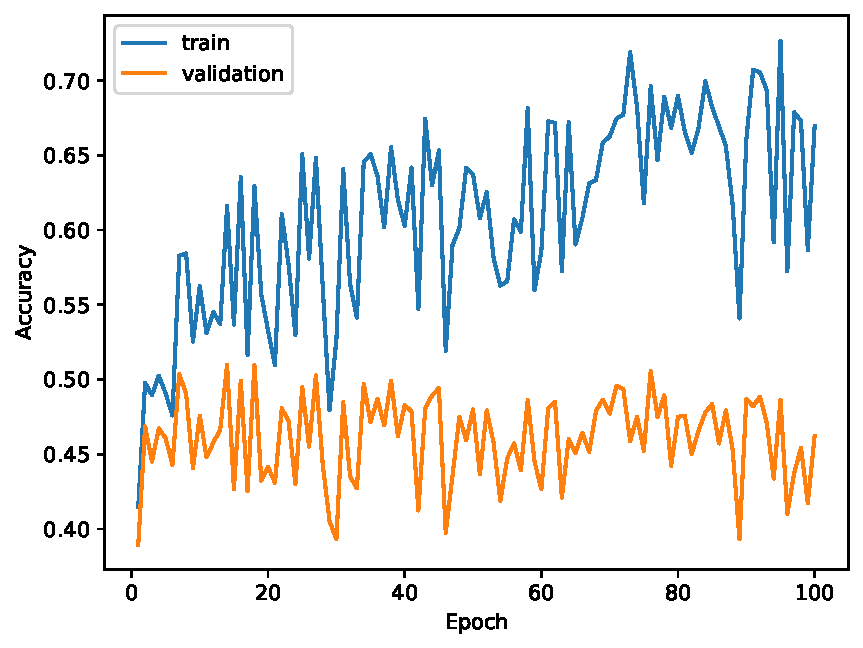
\includegraphics[width=0.4\textwidth]{images/Q1-logistic_regression-accs.pdf} 
    \caption{Train and validation accuracies of linear regression without regularization }
    \label{fig:no_reg_acc_log_reg}
\end{figure}

Accuracies obtained with $l_2$ regularization: \\
Performance on training set:  0.5683\\
Performance on validation set: 0.4972 \\
Performance on test set:  0.5053 \\


\begin{figure}[H]
    \centering
    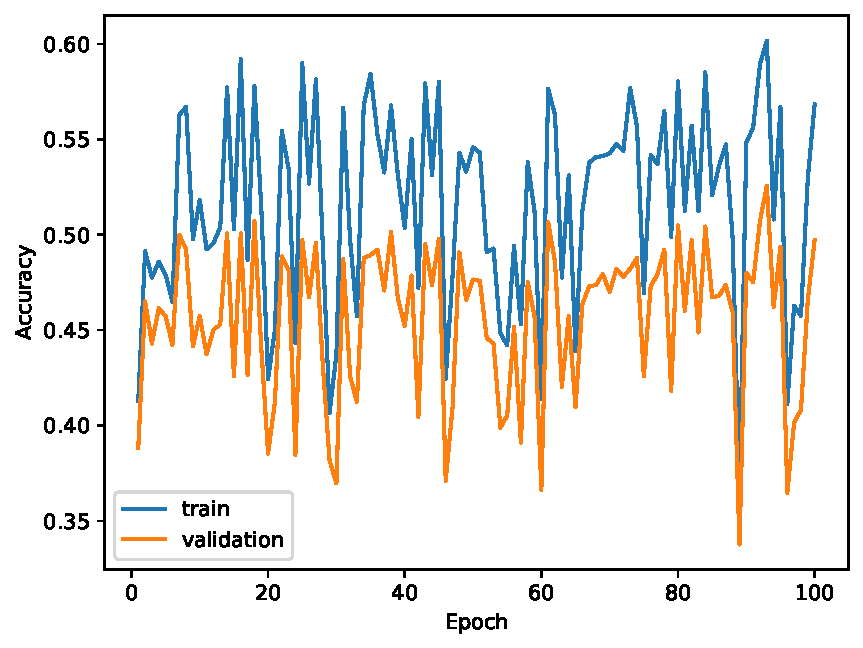
\includegraphics[width=0.4\textwidth]{images/Q1-logistic_regression-accs_with.pdf} 
    \caption{Train and validation accuracies of linear regression with regularization}
    \label{fig:dd}
\end{figure}

The performance on the training set is higher for the method without regularization. However, this is not the case for the test and validation set, leading to the conclusion that we do not achieve a better performance without regularization. Instead the discrepancy between the accuracies for training and validation set (see \ref{fig:no_reg_acc_log_reg}) set might indicate that overfitting is occuring.

\subsubsection{$\ell_2$ Norms}
\begin{figure}[H]
    \centering
    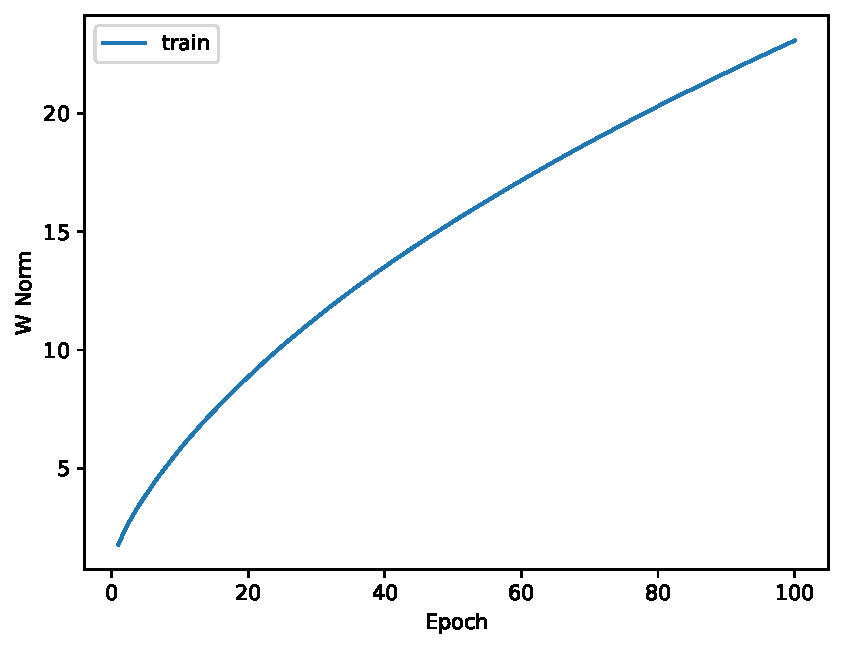
\includegraphics[width=0.4\textwidth]{images/Q1-logistic_regression-w_norms.pdf} 
    \caption{$\ell_2$ norms of the Weights-Matrix during the epochs without regularization }
    \label{fig:dd}
\end{figure}

\begin{figure}[H]
    \centering
    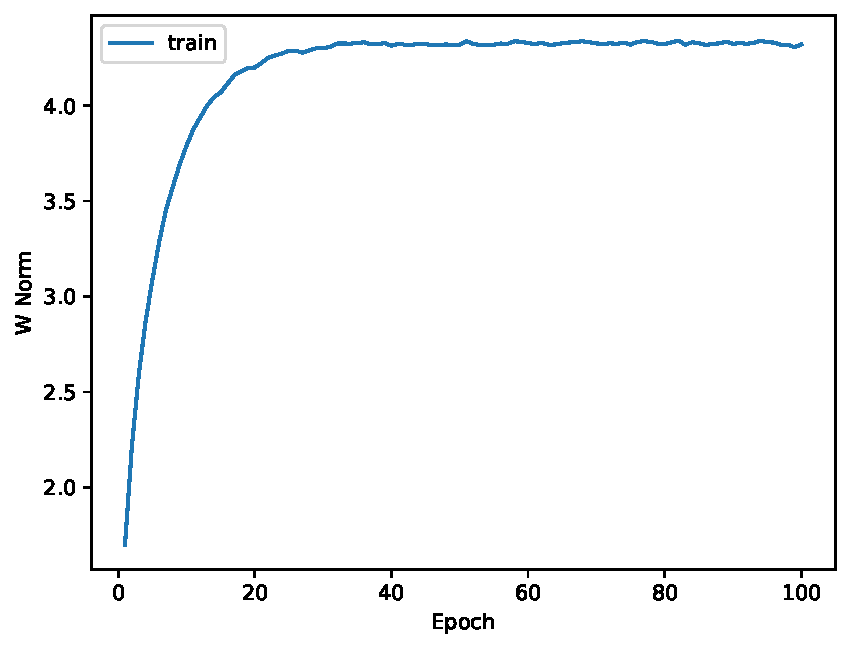
\includegraphics[width=0.4\textwidth]{images/Q1-logistic_regression-w_norms_with.pdf} 
    \caption{$\ell_2$ norms of the Weights-Matrix during the epochs with regularization}
    \label{fig:dd}
\end{figure}

It can bee seen that without regularization the $\ell_2$-norm of the weights grows almost constant from point onward, while when regularization is introduced the $\ell_2$-norm of the weights stays relatively constant after reaching a certain value.

\subsubsection{$\ell_1$ vs $\ell_2$ Regularization}

When using $\ell_1$ regularization instead of $\ell_2$ one would expect the weight-matrix to become sparse. Some values in the weight-matrix would become zero. In $\ell_2$-regularization the values in the weight-matrix do not necessarily become zero but smaller overall.

\subsection{Multi-Layer Perceptron}